\section{Process View}
De process view van het 4 + 1 model dient om het run-time gedrag van het systeem in beeld te brengen \parencite{4p1Model}.
In deze sectie wordt er gekeken hoe het ophalen van de data vanuit de backend werkt.
Verder wordt er ook gekeken hoe de data gerenderd wordt in de frontend.

\subsection{Backend}
Om het proces van het ophalen van de data in beeld te krijgen is er gebruikgemaakt van een sequencediagram.
In figuur \ref{fig:SequenceDiagramItemValueWithChildren} (vergrote afbeelding is te zien in \ref{appendix:SequenceDiagramItemValueWithChildren}) is te zien dat er 4 lagen zijn. 
Dit zijn de controller, datahandler, handler en repository.
De logica om te bepalen of het een succesvolle request was zit in de datahandler.
De verschillende handlers handelen de buisness logica af.
En als laatste is er de repository die de data uit de database haalt.

\whitespace
\begin{graphic}
    \captionsetup{type=figure}
    \caption{Sequencediagram ItemValue}
    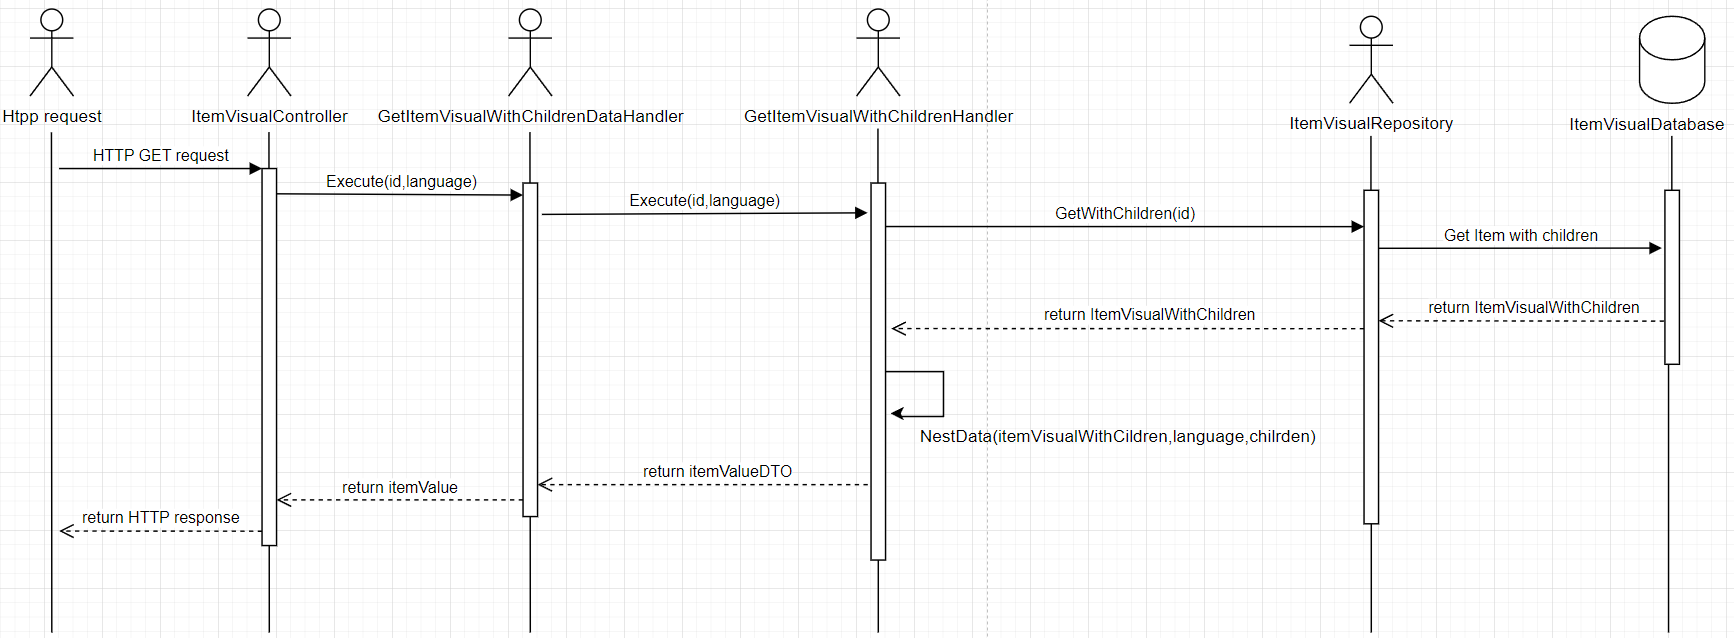
\includegraphics[scale=0.28]{SequenceDiagramItemValueWithChildren.png}
    \label{fig:SequenceDiagramItemValueWithChildren}
\end{graphic}

\newpage
\subsection{Frontend}
\label{sec:FrontendProcessView}
Om de geneste structuur van het datamodel te renderen wordt er gebruikgemaakt van 2 verschillende component types.
Deze component types worden appart toegelicht om een beter beeld te schetsen.

\whitespace[2]
\textbf{Type 1: Implementatie componenten}

\whitespace
Het eerste type componenten is het component dat daadwerkelijk de data rendered.
Deze componenten pakken de \textit{fields} van het \textit{item} en renderen dit op de frontend.
Als voorbeeld is er een stukje van de Snakeware site gepakt om dit beter toe te lichten (zie figuur \ref{fig:SingleComponent})
In dit voorbeeld wordt het titel field  gebruikt om de titel van het component te renderen.
En hetzelfde wordt ook gedaan voor het nummer en de body van het component.

\begin{graphic}
    \captionsetup{type=figure}
    \caption{Visualisatie implementatie component}
    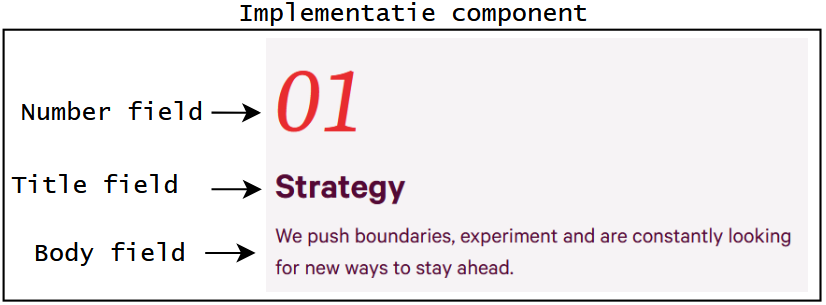
\includegraphics[scale=0.4]{ExampleDiffrentFrontendTypes.png}
    \label{fig:SingleComponent}
\end{graphic}

\whitespace[2]
\textbf{Type 2: Containers}

\whitespace
Omdat de datastructuur meerder componenten moet kunnen groeperen wordt er gebruikgemaakt van containers.
Containers zijn generieke componenten die een of meerdere implementatie componenten of meerdere containers kan renderen kan renderen.
Door het gebruik van een generieke structuur is het mogelijk om elke complexe datastructuur te renderen zonderen enige aanpassingen te maken aan het model zelf.
%
%
% Omdat Implementatie componenten in elkaar genest kunnen zitten wordt er ook gebruik gemaakt van containers.
% Verder kunnen containers ook meerdere containers renderen.
% Door dit te doen kunnen complexe structuren gerenderd.
Om hier een beter beeld bij te schetsen is het vorige voorbeeld (zie figuur \ref{fig:SingleComponent}) uitgebreid.
De uitgebreide versie is te zien in figuur \ref{fig:MultipleComponents}.
Verder is er in figuur \ref{fig:ExampleDataStructure} een voorbeeld gemaakt van een versimpelde site architectuur.
Normaliter bevatten de \textit{content container} ook meerdere containers en implementatie componenten.
Deze zijn weggelaten om mee voor meer duidelijkheid te geven aan het figuur.
Verder is het figuur in de rechterkant van elke container en implementatie component een nummer te zien.
Deze nummers laten zien in welke volgorde de componenten gerenderd worden.

\whitespace
\begin{graphic}
    \captionsetup{type=figure}
    \caption{Visualisatie containers}
    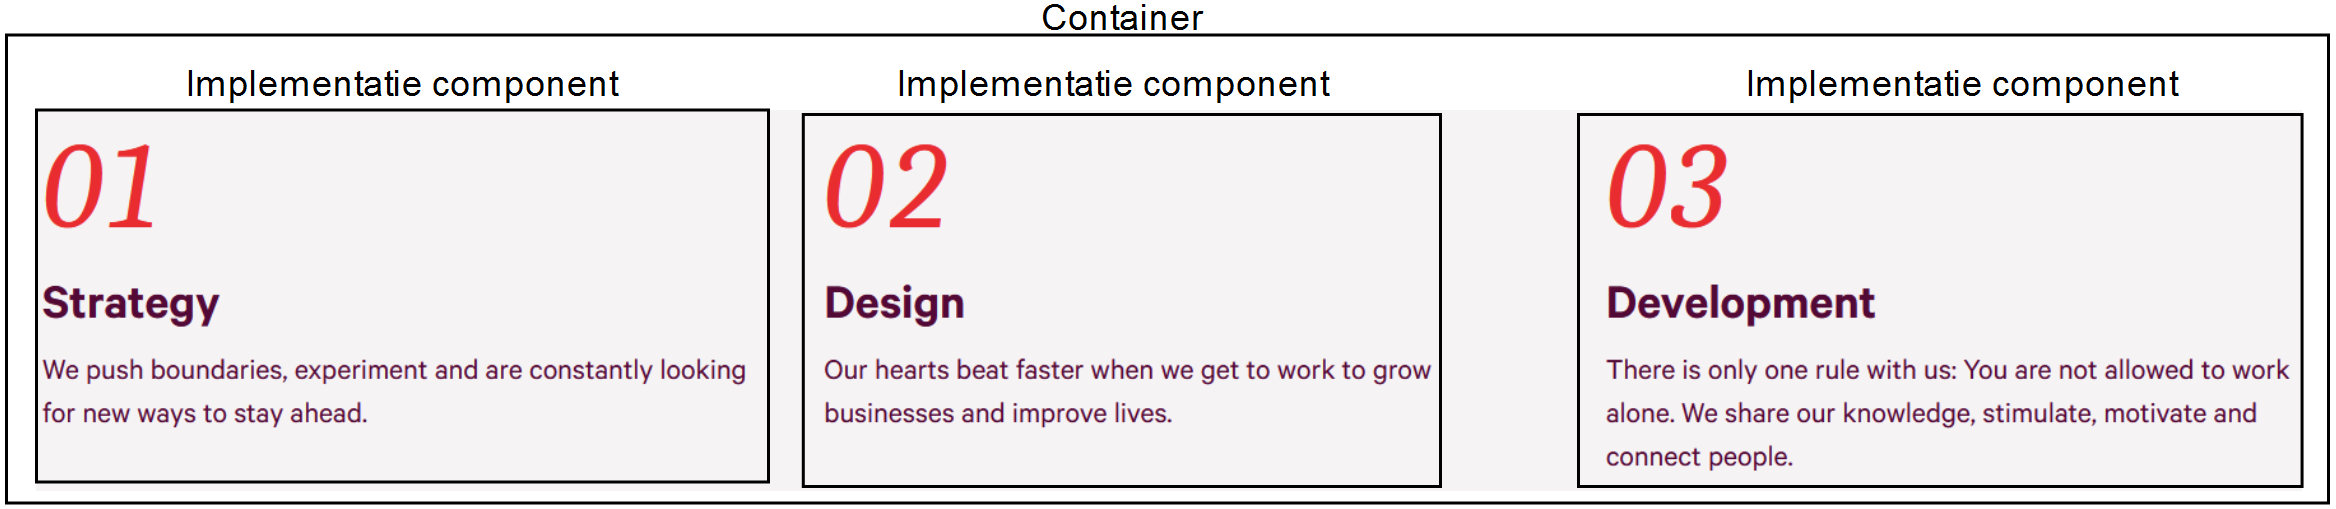
\includegraphics[scale=0.27]{ExampleContainerFrontend.png}
    \label{fig:MultipleComponents}
\end{graphic}

\newpage
\whitespace
\begin{graphic}
    \captionsetup{type=figure}
    \caption{Visualisatie containers}
    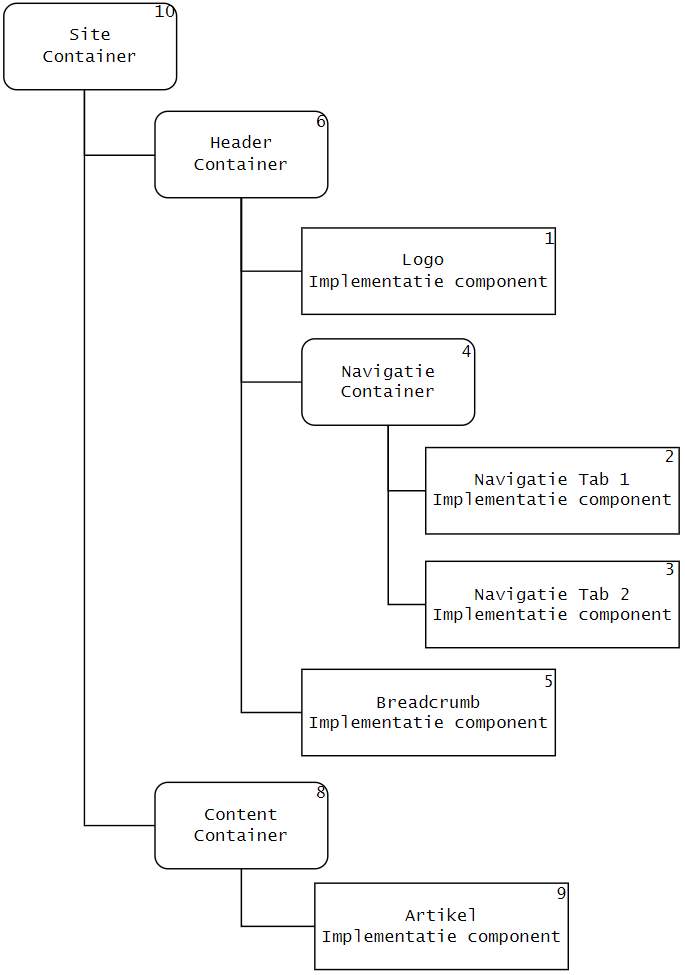
\includegraphics[scale=0.4]{ExampleDataStructure.png}
    \label{fig:ExampleDataStructure}
\end{graphic}

\whitespace
Figuur \ref{fig:FlowchartFrontend} laat zien hoe de frontend omgaat met deze containerstructuur.
Na het ophalen van de data van de api wordt de root container gerendered.
Eerst wordt er gekeken of het huidige object 1 of meer items heeft.
Daarna wordt er gecontroleerd of het item een valide implementatie component heeft.
Als het item een container is dan wordt deze recursief gerenderd.
Dit wordt gedaan tot dat alle items gerenderd zijn.

\whitespace
\begin{graphic}
    \captionsetup{type=figure}
    \caption{flowchart diagram frontend}
    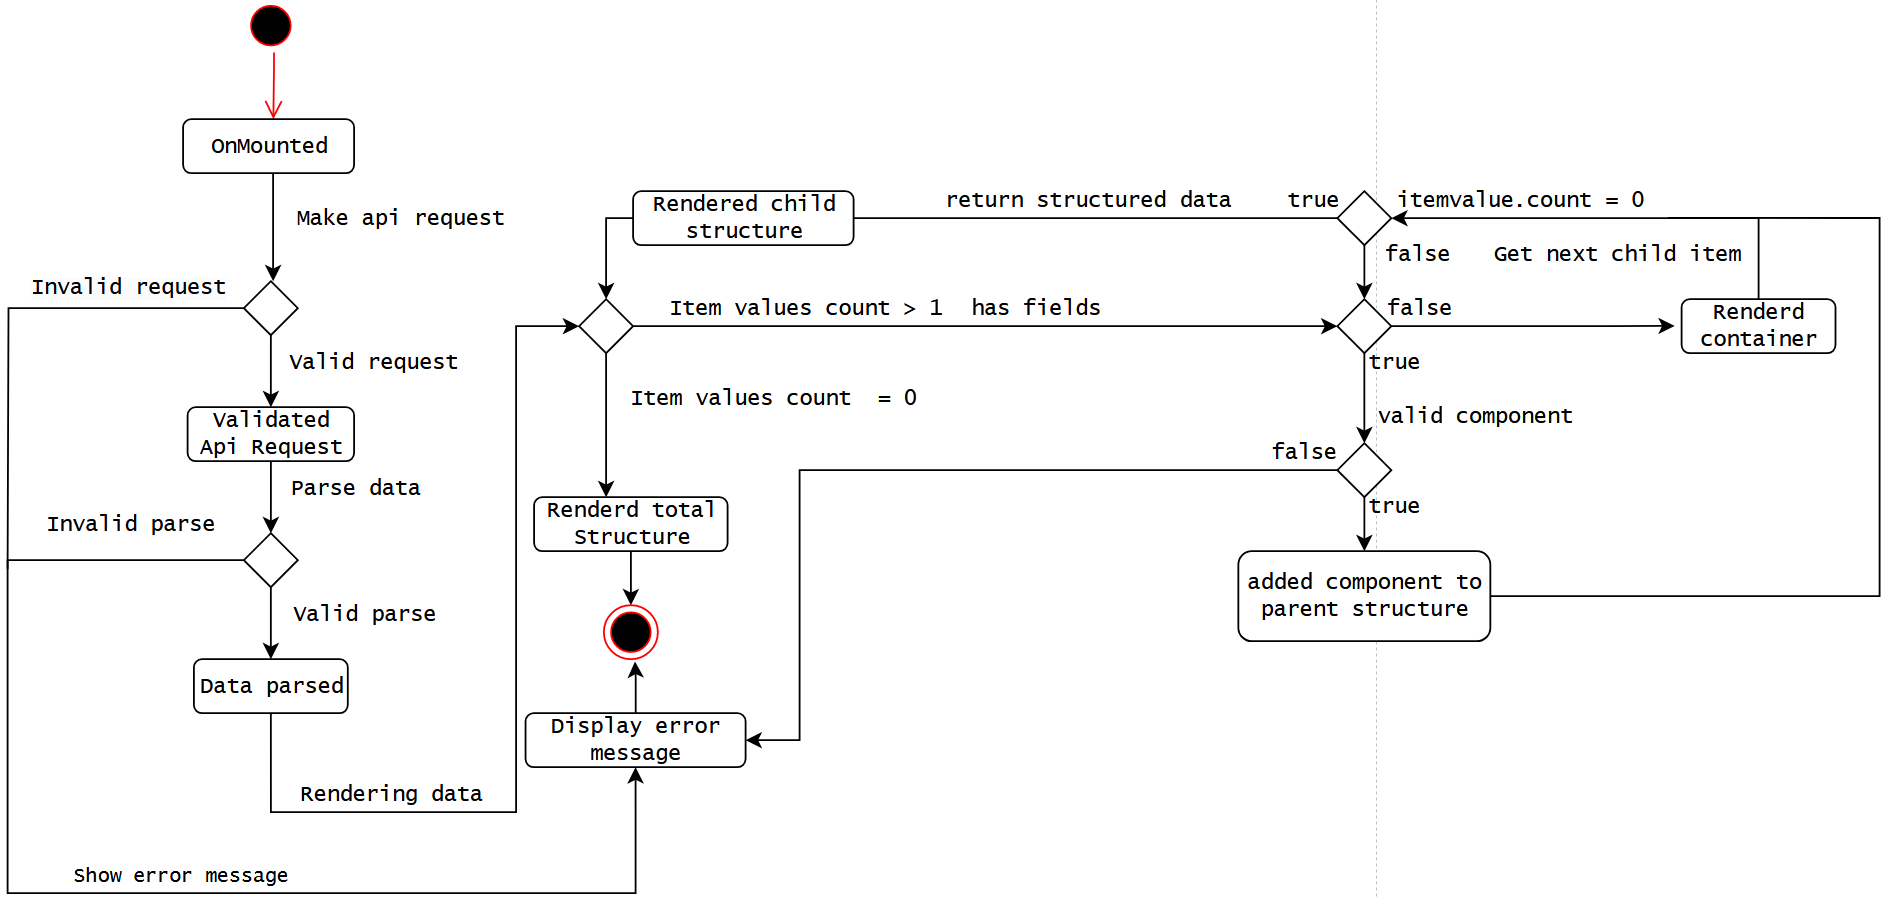
\includegraphics[scale=0.34]{FlowchartFrontend.png}
    \label{fig:FlowchartFrontend}
\end{graphic}
